\chapter{Boosted Decision Trees}\label{cha:bdt}

As shown in \cref{sec:event_selection:yields} only a small fraction of all events which are analyzed originate
from the signal process.
All other events are produced by background processes.
Since the goal is to extract information from the signal, one challenge of this analysis is to reduce
background contributions as much as possible.

An established approach to separate signal and background is to restrict observables to a given range.
The observables and thresholds (cuts) are selected and optimized by hand, which can be a tedious task.
However, it is very easy to implement in the analysis and the effect of each threshold is easily comprehensible.
Multiple observables are used to reject different types of background contributions.
Such an approach is described in \cref{cha:event_selection}.

Another way to achieve separation between signal and background is with the help of machine learning (ML) algorithms.
The most common ML algorithms used in high energy physics are \emph{boosted decision trees} (BDTs) and neural networks.
In this thesis an approach to use BDTs for the analysis of the \Httll{} process in the 2015 + 2016 dataset is developed.
This chapter focuses on the general and theoretical aspects of boosted decision trees, while the application of BDTs in this analysis
is discussed in \cref{cha:mva}. For this the ROOT~\cite{ROOT} library TMVA~\cite{TMVA} is used.

First, decision trees are introduced in \cref{sec:bdt:decision_trees}, since they are the foundation of BDTs.
Then, the concept of boosting is explained in \cref{sec:bdt:boosting} and different boosting algorithms are presented.
Finally, a summary of BDT parameters is given in \cref{sec:bdt:hyperparameters}.

The contents of this chapter are based on Refs.~\cite{Hastie2009,TMVA}.

\section{Introduction to Machine Learning}\label{sec:bdt:intro}

Machine learning has two different applications.
It can be used to assign class labels to the data points (\emph{classification}) or to predict
an outcome encoded in a continuous variable via \emph{regression}.
For this analysis classification is used, since the goal is to split the events in signal and background.
In general, there can be an arbitrary amount of output classes, but to simplify the discussion this chapter focuses
only on two-class problems in the aspect of splitting signal and background events.

Both types of machine learning rely on the same principle.
First, a model has to be trained with data, the so-called \emph{training set}, where the correct result is already known.
The data used can either come from measurements or simulation.
After the model is trained it can be applied to another set of data.
It is important that the data which was used for training the model is not used in the real measurement, because
the model would perform better on the training set than on a independent data set.
This issue is discussed in more detail in \cref{sec:mva:kfold-xval}.

It can happen that a model performs much worse on a independent data set than on the training set.
This effect is known as \emph{overtraining}.
In this case the model was trained too much and is sensitive to statistical fluctuations in the training set.
Overtraining can be avoided if the correct parameters of the model are chosen.

\section{Decision Trees}\label{sec:bdt:decision_trees}

A decision tree has a binary-tree-like structure as shown in \cref{fig:bdt:dt}.
The root node contains all signal and background events.
All events are sorted into two subnodes, based on a certain observable (input variable) and threshold.
Now the splitting procedure is recursively applied again on each of the subnodes, until a
stopping criterion is met.
The final notes are labeled as signal- or background-like, depending on the majority of their contents.
A signal-like node results in an output of $+1$ of the decision tree, a background-like node yields $-1$.
After the decision tree is built it can be applied to data events, where it classifies the data events as either
signal- or background-like.

\begin{figure}[htb]
    \begin{center}
        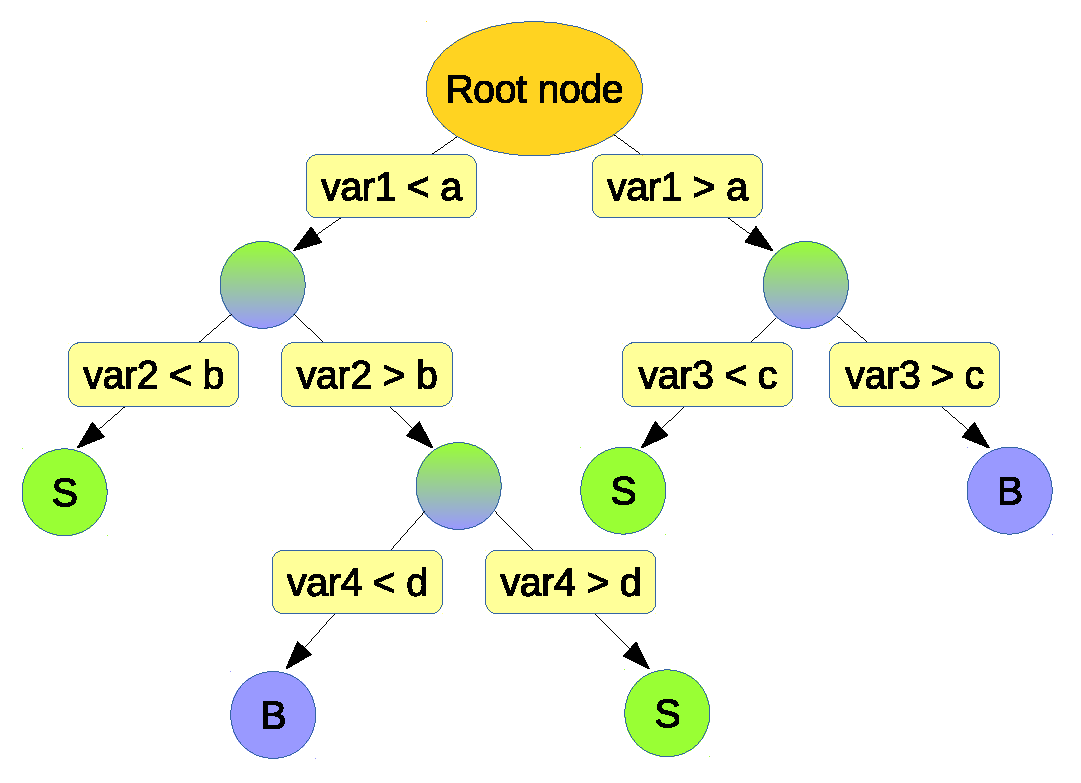
\includegraphics[width=0.8\linewidth]{./figures/bdts/DT.eps}
        \caption{Exemplary structure of a decision tree with a depth of $3$.
                 Signal- and background-like nodes are labeled with a $S$ and $B$.}\label{fig:bdt:dt}
    \end{center}
\end{figure}

A decision tree can be interpreted as a function $G(x_i)$, which takes multiple input variables of one event $x_i$, with
the following output:
\begin{equation}
    \label{eq:dt}
    G(x_i) =
    \begin{cases}
        +1 & \text{signal-like} \\
        -1 & \text{background-like}
    \end{cases} \,.
\end{equation}
If some signal and background events have similar properties, the decision tree cannot reach a perfect performance.
Some signal events are classified as background events and the other way around.
This is called \emph{misclassification}.
A good decision tree has only a small number of misclassified events.

\subsection{Growing a decision tree}\label{sub:bdt:dt:growing}

The process of deciding which observable and threshold is used to split each subnode
is called \emph{growing} or \emph{building} a decision tree.
The goal of the splitting is to improve the pureness in of either signal or background events in the subnodes with respect to the parent node.

The purity $p$ of a node is defined as
\begin{equation}
    \label{eq:purity}
    p = \frac{s}{s+b}\,,
\end{equation}
where $s$ is the number of signal events and $b$ the number of background events.
A node with only signal events has the purity of one, a node containing only background events has the purity of zero.

Based on the purity of the node a separation criterion $Q$ is calculated.
The separation criterion is a function which reaches its maximum when the node is fully mixed, i.e.\ for $p = 0.5$.
Below some examples of different separation criteria are given.
\begin{itemize}
    \item Gini index: $Q = p (1-p)$
    \item Cross entropy: $Q = -p  \log(p) - (1 - p) \log (1 - p)$
    \item Misclassification error: $Q = 1 - \max (p, 1 - p)$
\end{itemize}
To increase the pureness of a node the increase of the separation criterion has to be optimized.
The change of the separation criterion for a selected input variable $v$ and threshold $t$
is the difference between the sum of the new separation criteria, weighted
by the relative fraction of events, and the separation criterion of the parent node,
\begin{equation}
    \Delta Q(v, t) = \sum_{i=1,2} \frac{n_i}{n_\text{parent}} Q_i (v, t) - Q_\text{parent} \,.
\end{equation}
Here $n_i$ is the number of events in each subnode, $n_\text{parent}$ the number of events in the parent node,
$Q_i$ the value of the separation criterion of each subnode, and $Q_\text{parent}$ the value of the separation criterion
in the parent node.
The maximum value of $\Delta Q$ is selected by considering all given input variables.
For each variable a scan over the its range in the training set is performed.
Since there is a finite amount of events in each node it is possible to change the thresholds in such a way that after
each change only one event is sorted differently.
However, this would need large amounts of computational power and is therefore not feasible in most applications.
Thus, a common approach is to only test a certain amount of thresholds, which are distributed over the whole range
of the variable.

In principle the splitting can go on until each node contains only one event, but this would lead
to an overtrained decision tree.
This can be prevented by \emph{pruning} the decision tree, a process where nodes with low numbers of events are combined.
Another way to stop growing the decision tree is to impose some cancellation criteria, so that the fine splitting
does not happen in the first place.
For example the maximal depth of the tree can be limited or nodes are only split again if they
contain a certain number of events.

\subsection{Comparison to Selection Cuts}\label{sub:bdt:dt:comparison}

Using decision trees has some advantages over the standard approach (denoted as cut-based analysis, CBA) of sequentially requiring thresholds on different
observables.
Usually all events which do not satisfy one requirement are discarded immediately.
In decision trees all events are kept.
It can happen that a signal event is first sorted into a background-like node, but later on the node is split again and
the event falls into a signal-like node.
Therefore, decision trees should provide an improved classification performance.
This can be visualized by looking at the space which is spanned by the input variables.
The cut-based approach selects only one hypercube in the
feature-space\footnote{In machine learning, the input variables are called \emph{features}.}.
Decision trees can select multiple hypercubes in this space.

Additionally, decision trees (and also other machine-learning models) are also sensitive to correlations
between the input variables, which enables the decision trees to better classify events.

\subsection{Disadvantages}\label{sub:bdt:dt:disadvantages}

Decision trees are not a perfect solution, they also have their drawbacks.
In machine learning generally all models have a certain dependence on statistical fluctuations of the training set.
If the training set is split into two sets and two individual decision trees are trained, they should in principle have
a similar structure.
However, due to statistical fluctuations one variable and threshold could be selected differently, which could lead
to a completely different structure of one decision tree.

Also, decision trees are \emph{weak classifiers}, i.e.\ they provide only a performance slightly better than random guessing.

However, there are concepts which provide substantial improvements in both of those areas.
One method is the co-called \emph{boosting}, which is introduced in the next section.

\section{Boosting}\label{sec:bdt:boosting}

The idea of boosting is to combine many weak classifiers into a powerful \emph{committee}.
This increases the performance compared to using only one decision tree.
It is a very powerful way of improving the separation power of decision trees while
simultaneously reducing the probability of overtraining.

The general concept of boosting is as follows.
First one decision tree is trained on the initial training set.
Weights are assigned to each event based on the output of the decision tree.
If an event is misclassified a higher weight is assigned to it.
Now, a new decision tree is trained on the weighted training set.
Because previously misclassified events have a higher weight they have more impact on the current training step
than corrctly classified events.
This procedure is repeated multiple times, until a maximum number of iterations is reached.
The final output is a combination of the output of all decision trees which were trained.
This combination known as the \emph{boosted decision tree}.

There are different algorithms which implement this general boosting strategy.
In the next sections first the \emph{AdaBoost} algorithm is introduced, which is a simple boosting algorithm.
It can be shown, that AdaBoost is a specific case of a general concept, which leads then to the second
boosting algorithm which is discussed, the \emph{gradient boost}.

\subsection{AdaBoost}\label{sub:bdt:boosting:adaboost}

The AdaBoost algorithm~\cite{AdaBoost} was developed initially in 1997 by Yoav Freund and Robert Schapire.
Until today it is one the most popular boosting algorithms.

Let $x$ be a set of $N$ input events and $y$ the corresponding output values.
Single values are referred to as $x_i$ and $y_i$ with $i \in \{1, \ldots, N\}$, respectively.
The classifier, in this case the decision tree, is denoted as $G(x_i)$, with $G(x_i) \in \left\{ -1,1 \right\}$.

In the beginning each event is assigned a weight $w_i$, where
\begin{equation}
    w_i = \frac{1}{N} \,.
\end{equation}
For each boosting step $m$ the classifier is trained with the training events using the weights $w_i$.
After the training the misclassification error, $\err_m$, is calculated, which is the weighted avereage of the number of misclassified events,
\begin{equation}
    \err_m = \frac{\sum_{i_1}^N w_i I(y_i \neq G_m(x_i))}{\sum_{i_1}^N w_i} \,.
\end{equation}
Here the indicator function $I$ is used, which is defined as follows:
\begin{equation}
    I(cond.) =
    \begin{cases}
        1 & \text{if $cond.$ is true} \\
        0 & \text{else}
    \end{cases} \,.
\end{equation}
The boost weight $\alpha_m$ is calculated,
\begin{equation}
    \alpha_m = \log \frac{1 - \err_m}{\err_m} \,.
\end{equation}
It regulates how much the weights are altered for each misclassified event in the next iteration.
The weights which are used in the next boosting step $m+1$ are set in the following way:
\begin{equation}
    w_i^{m+1} = w_i^{m} \exp \left[ \alpha_m I \left(y_i \neq G_m(x_i)\right) \right] \,.
\end{equation}
Only the weights of the events which are misclassified are altered.
After the maximum number of boosting iterations, $M$, the final output $G(x)$ of the boosted decision tree
can be calculated.
The output of all decision trees weighted by the boost weight of this step is summed up,
\begin{equation}
    \label{eq:bdts:output_ada}
    G(x) = \frac{1}{M} \sum_{m=1}^M  \alpha_m G_m(x) \,.
\end{equation}
In contrast to the discrete output of single decision trees the combined output can have a real value between $-1$ and $1$.

The learning rate can be adjusted by replacing the boost weight $\alpha_m$ with $\alpha_m^\beta$, where
$\beta$ ($0 < \beta \leq 1$) is the so-called AdaBoost-beta.
A small value for $\beta$ reduces the risk of overtraining but may reduce the performance.

AdaBoost performs best on weak classifiers.
This means that the maximum depth of decision trees should be limited to low numbers, if they are used in combination with
AdaBoost.
\cref{fig:bdt:adaboost_testerror} shows the test error, a quantity similar to the misclassification error but evaluated on
an independent test set, as a function of the number of boosting iterations.
The decision tree which is used has a depth of only one.
Its error rate is around $0.45$, which is only slightly better than random guessing, where the error rate is $0.5$.
When boosting is used, the error rate decreases to only $0.05$, which is a huge improvement.
The boosted decision tree also performs better than one single decision tree with 244 nodes, whose error rate is still at $0.25$.
After approximately 300 boosting iterations there is only little or no performance gain at all.

\begin{figure}[htb]
    \centering
    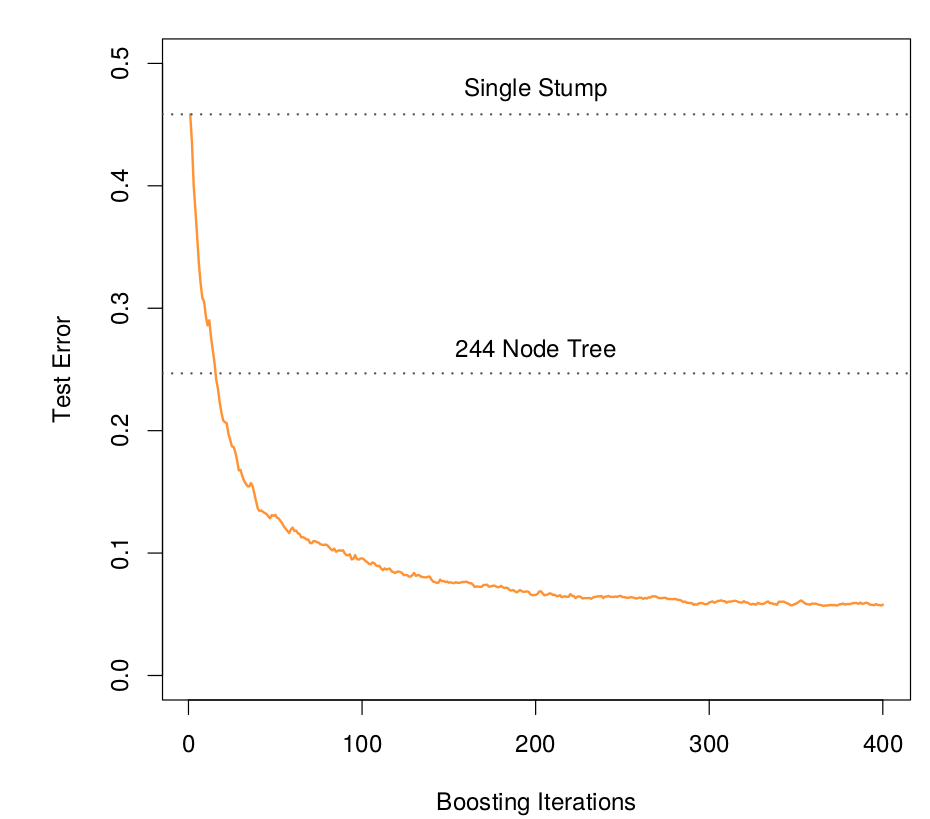
\includegraphics[width=0.7\textwidth]{./figures/bdts/adaboost_testerror.png}
    \caption{Test error of a decision tree with a depth of one, boosted with AdaBoost, as the function of the number of boosting iterations.
             The test errors of the single decision tree (Single Stump) and a decision tree with 244 nodes (244 Node Tree) are also indicated~\cite{Hastie2009}.}\label{fig:bdt:adaboost_testerror}
\end{figure}

\subsection{A General Approach to Boosting}\label{sub:bdt:boosting:general}

The concept of boosting can be generalized.
Building a committee of decision trees like in \cref{eq:bdts:output_ada} can be interpreted as
fitting an additive expansion in a set of functions which build a basis.
For AdaBoost those basis functions are the individual decision trees $G_m(x)$.
A general basis function expansion can be written as
\begin{equation}
    f(x) = \sum_{m=1}^M \beta_m b(x; \gamma_m) \,,
\end{equation}
where $f(x)$ is the function to approximate, $\beta_m$ the expansion coefficients, and $b(x; \gamma_m)$
the base function with the input observables $x$ as argument and $\gamma_m$ as parameter.

To obtain the best approximation the optimal values of $\beta_m$ and $\gamma_m$ need to be found.
A measure to quantify the agreement between the model and the training data is needed.
Functions which provide such a measure are called \emph{loss functions} and are denoted here as $L(y, f(x))$.
They take the output values, $y$, and the approximated function, $f(x)$, as arguments.
Loss functions are discussed below in more detail.

The optimal values for $\beta_m$ and $\gamma_m$ can be found by minimizing the loss function:
\begin{equation}
    \label{eq:bdts:optimization_loss_function}
    \min_{{\{\beta_m, \gamma_m\}}_{m=1}^M} \sum_{i=1}^{N} L \left( y_i, \sum_{m=1}^{M} \beta_m b(x_i; \gamma_m) \right) \,.
\end{equation}

\subsubsection{Forward Stagewise Additive Modeling}\label{subsub:bdt:boosting:forward_modeling}

The optimization described in \cref{eq:bdts:optimization_loss_function} is computationally very expensive, since
this is a optimization in a high-dimensional space.
However, the optimization can be approximated with an iterative approach, known as \emph{forward stagewise additive modeling}.
If the approximation up to step $m-1$ is already known, the parameters and coefficient of step $m$ can be found
in the following way, while keeping the parameters and coefficients of the previous base functions constant:
\begin{equation}
    (\beta_m, \gamma_m) = \arg \min_{\beta, \gamma} \sum_{i=1}^N L(y_i, f_{m-1}(x_i) + \beta b(x_i, \gamma)) \,.
\end{equation}
After finding $\beta_m$ and $\gamma_m$ the approximated function at step $m$ can be build with
\begin{equation}
    f_m(x) = f_{m-1}(x) + \beta_m b(x_i, \gamma_m)
\end{equation}
The first base function, $f_0$, is usually initialized with zero.

It can be shown that the AdaBoost algorithm is equivalent to forward stagewise additive modeling if an exponential
loss function,
\begin{equation}
    L(y, f(x)) = \exp \left[ - y f(x) \right] \,,
\end{equation}
is used~\cite{Hastie2009}.
The base functions are here the individual decision trees, $G_m(x)$.
This connection is not trivial and was only observed several years after the AdaBoost algorithm was
developed.

\subsubsection{Loss functions}\label{subsub:bdt:boosting:lossfunction}

Loss functions quantify the discrepancy between a model and the correct output value.
They depend on the margin, which is defined as $y \cdot f(x)$.
The margin in classification problems has the analogous role of the residual $y - f(x)$ in regressions.
A positive margin indicates that the event was classified correctly, a negative margin signals misclassification.
The boundary between an correctly classified event and misclassified event is at $f(x) = 0$.

Loss functions need to be monotone decreasing, so that misclassified events are penalized by a high value
of the loss function.
A list of common loss functions is given below.
\begin{itemize}
    \item Misclassification: $I(\sign(f) \neq y)$
    \item Exponential: $\exp(-yf)$
    \item Binomial Deviance: $\log (1 + \exp(-2yf))$
    \item Squared Error: ${(y-f)}^2$
    \item Support Vector\footnote{The label ${}_+$ denotes that negative values are set to zero.}: ${(1-yf)}_+$
\end{itemize}
They are shown as a function of the margin in \cref{fig:bdt:loss_functions}.

\begin{figure}[htb]
    \centering
    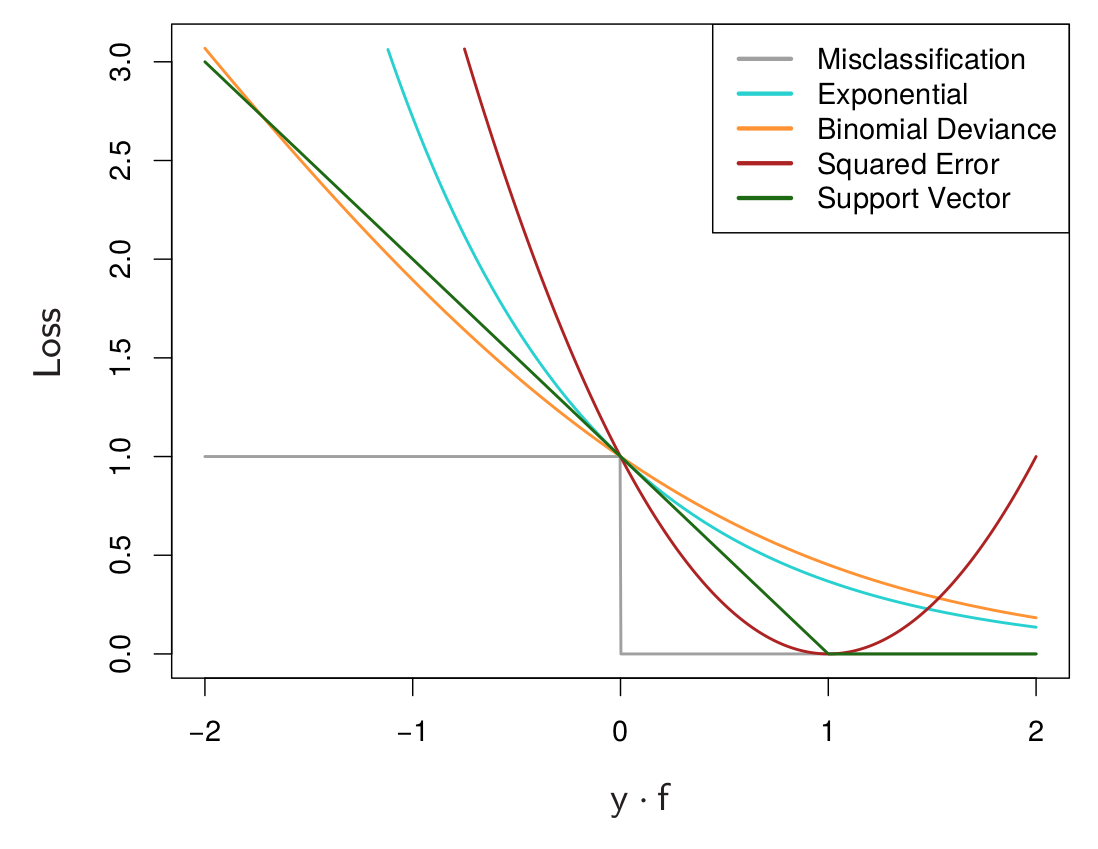
\includegraphics[width=0.7\textwidth]{./figures/bdts/loss_functions.png}
    \caption{Value of different loss functions as a function of the margin $y \cdot f$.
             The functions are scaled in such a way that they pass through $(0, 1)$~\cite{Hastie2009}.}\label{fig:bdt:loss_functions}
\end{figure}

Both the exponential loss and binomial deviance can be seen as a continuous approximation of the misclassification loss,
which is a step function.
For an increasing negative margin the penalty of the binomial deviance grows in a linear fashion, for the exponential loss
it grows exponentially.
The binomial-deviance loss is more robust compared to the exponential loss, because misclassified events have less impact.
The squared-error loss is not a good replacement for the misclassification loss, since correctly classified events
above a margin of one receive an increased penalty.

\subsection{Gradient Boost}\label{sub:bdt:boosting:gradient_boost}

The \emph{gradient boost} algorithm is a boosting algorithm which can use any differentiable loss function.
It applies the approach of forward stagewise additive modeling.
The loss function is minimized via the \emph{gradient descent} algorithm, a popular algorithm used to find the minimum
of a function, in function space.
The gradient, which is used for the minimization, is calculated as follows:
\begin{equation}
    g_{im} = {\left[ \frac{\partial L(y_i, f(x_i))}{\partial f(x_i)} \right]}_{f(x_i) = f_{m-1}(x_i)} \,.
\end{equation}
However, this leads to an issue.
The gradient needs to be known for every point in the space of the input observables, $x_i$.
But since those are provided from a finite amount of training data, the gradient is only known at those points.
The solution is to use a regression tree for the estimation of values between the training data points.

The learning rate can be adjusted in a similar way like for the AdaBoost algorithm.
A parameter $\nu$ ($0 < \nu \leq 1$) called \emph{shrinkage} is introduced, which acts as the learning rate.
The output of every decision tree is scaled with the shrinkage,
\begin{equation}
    f_m(x) = f_{m-1}(x) + \nu \beta_m b(x_i; \gamma_m) \,.
\end{equation}

\section{Hyperparameters}\label{sec:bdt:hyperparameters}

Throughout this chapter several parameters of boosted decision trees are mentioned.
Those parameters are not determined automatically and need to be set by the user.
In the machine-learning community, they are also known as \emph{hyperparameters}.
A large part of the next chapter is dedicated to find optimal values for those parameters.
This section gives an overview of the hyperparameters and a general recommendation which values lead to the best
performance.
For some parameters a short identification string is introduced, which makes it easier to refer to
those parameters late on.

To grow a single decision tree different thresholds for the observables are tested.
The number of grid points in the range of the observable needs to be set.
Studies suggest that a value of $20$ is high enough to get a good splitting performance.
A notable increase of the separation power with a higher number of grid points could not be seen~\cite{TMVA}.
Therefore, this analysis does not optimized the number of grid points but uses the suggested value.

For the cancellation criteria the maximum depth of the tree (\texttt{MaxDepth}) and the minimum number of events in one node
given as the percentage w.r.t.\ the total event count (\texttt{MinNodeSize}) are used.
Since boosting works best with weak classifiers, a small amount of trees should be chosen.
To prevent overtraining the minimum number of events in one node should not be to small.

For boosting first it has to be decided which boosting algorithm (\texttt{BoostType}) should be used.
In case of the gradient-boost algorithm the loss function has to set.
TMVA uses the binomial-deviance loss.
Also the number of single decision trees which are used during the boosting (\texttt{NTrees}) and the
learning rate (\texttt{Shrinkage} for gradient boost and \texttt{AdaBoostBeta} for AdaBoost) need to be set.
Generally a large number of trees and a low learning rate are preferred, since they decrease the chance of overtraining
and lead to a lower misclassification rate.
